\chapter{Clustering}  \label{clustering}
\NZ{I would be grateful if you could help me to choose an appropriate title for this chapter. It describes my approach to classify LJMs, its implementation, and the experiment I conducted to evaluate it.}

In Chapter~\ref{ch4}, we described our anti-unification algorithm to construct an anti-unifier from AUASTs of a pair of LJMs with a special attention to logging calls. Recall that the general point of this study is to provide a concise description of where logging calls happen in the source code by constructing structural generalizations that represent the detailed structural similarities and differences of LJMs. To this end, we should develop an algorithm that:
\begin{itemize} [leftmargin=.5in]
\item classifies AUASTs of LJMs into groups using a measure of similarity such that AUASTs in each group has maximum similarity with each other and minimum similarity to other ones.
%such that entities
\item abstracts AUASTs of each group into a structural generalization representing the similarities and differences between them.
%abstracts structural correspondences of ASTs
\end{itemize}

To construct an anti-unifier and to develop a measure of similarity, we can utilize the anti-unification algorithm presented in Chapter~\ref{ch4}. However, to produce structural generalizations from AUASTs of a set of LJMs a further should be taken, which is applying a clustering algorithm that would allow the classification of AUASTs into groups. To this end, we have developed a modified version of an agglomerative hierarchical clustering algorithm. 


Our hierarchical clustering algorithm (Section~\ref{meth-clustering}) is a bottom-up approach that starts with singleton clusters, where each contains one AUAST. In every iteration, it merges the closest clusters which are the clusters with maximum similarity between their AUASTs. We use the similarity function described in Section~\ref{meth-similarity} to measure similarity between each pair of AUASTs and then construct an anti-unifier via the anti-unification algorithm described in Section~\ref{meth-antiUnifier} when it is needed to merge two clusters. 

To evaluate our clustering approach, we have developed a tool atop the anti-unifier-building tool, and conducted an empirical study on our test suite. In Section~\ref{clustering-assessmentt}, we will describe our experimental study and discuss the results. 

%Figure~\ref{fig:meth_overview} shows an overview of the general process of our anti-unification technique, as will be described in the following sections.

\section{The Clustering tool} \label{clusteringTool}
%\subsection{Anti-unifying a set of AUASTs} \label{meth-clustering}
To anti-unify a set of AUASTs of LJMs, we have developed a modified version of a hierarchical agglomerative clustering algorithm as described below:
\begin{enumerate} [leftmargin=.3in]
\item Start with singleton clusters, where each cluster contains one AUAST
\item Compute the similarity between clusters in a pairwise manner
\item Adjust the similarity between a cluster pair to zero, if the anti-unification of their AUASTs does not allow anti-unifying log method invocation nodes with each other as the structures enclosing them are not corresponded. 
\item Find the closest clusters (a pair of clusters with maximum  similarity)
\item Merge the closest cluster pair and replace them with a new cluster containing the anti-unifier of AUASTs of the two clusters
\item Compute the similarity between the new cluster and all remaining clusters
\end{enumerate}
\begin{itemize} [leftmargin=.3in]
\item Repeat Steps 3, 4, 5, and 6 until the similarity between closest clusters becomes below a predetermined threshold value
\end{itemize}

In this algorithm, the similarity between a pair of clusters is defined as the similarity between their AUASTs which is computed through the algorithm described in Section.
The step 3 is inserted to prevent the combination of clusters when the usage of logging in their AUASTs has not been performed in the same way and they should be in separate clusters. Furthermore, the similarity threshold is determined through informal experimentation.

Figure~\ref{fig:overview2} illustrates the clustering process for classifying a set of 4 AUASTs. In the first iteration, the closest clusters, which are cluster 1 and cluster 2, are merged and replaced by cluster 5. If threshold value is determined as threshold A, the process will be terminated as the similarity between the closest clusters is below this threshold;if not, cluster 3 and cluster 5 will be merged and  replaced by cluster 6. However, the similarity between AUASTs of cluster 6 and 7 is zero, thus they should not be merged with each other. 


The $n \times n$ similarity matrix is shown in Figure~\ref{} where an element in row $i$ and column $j$ represents the similarity between the $i^{\text{th}}$ and the $j^{\text{th}}$ clusters .

\begin{figure} [H]
  \centering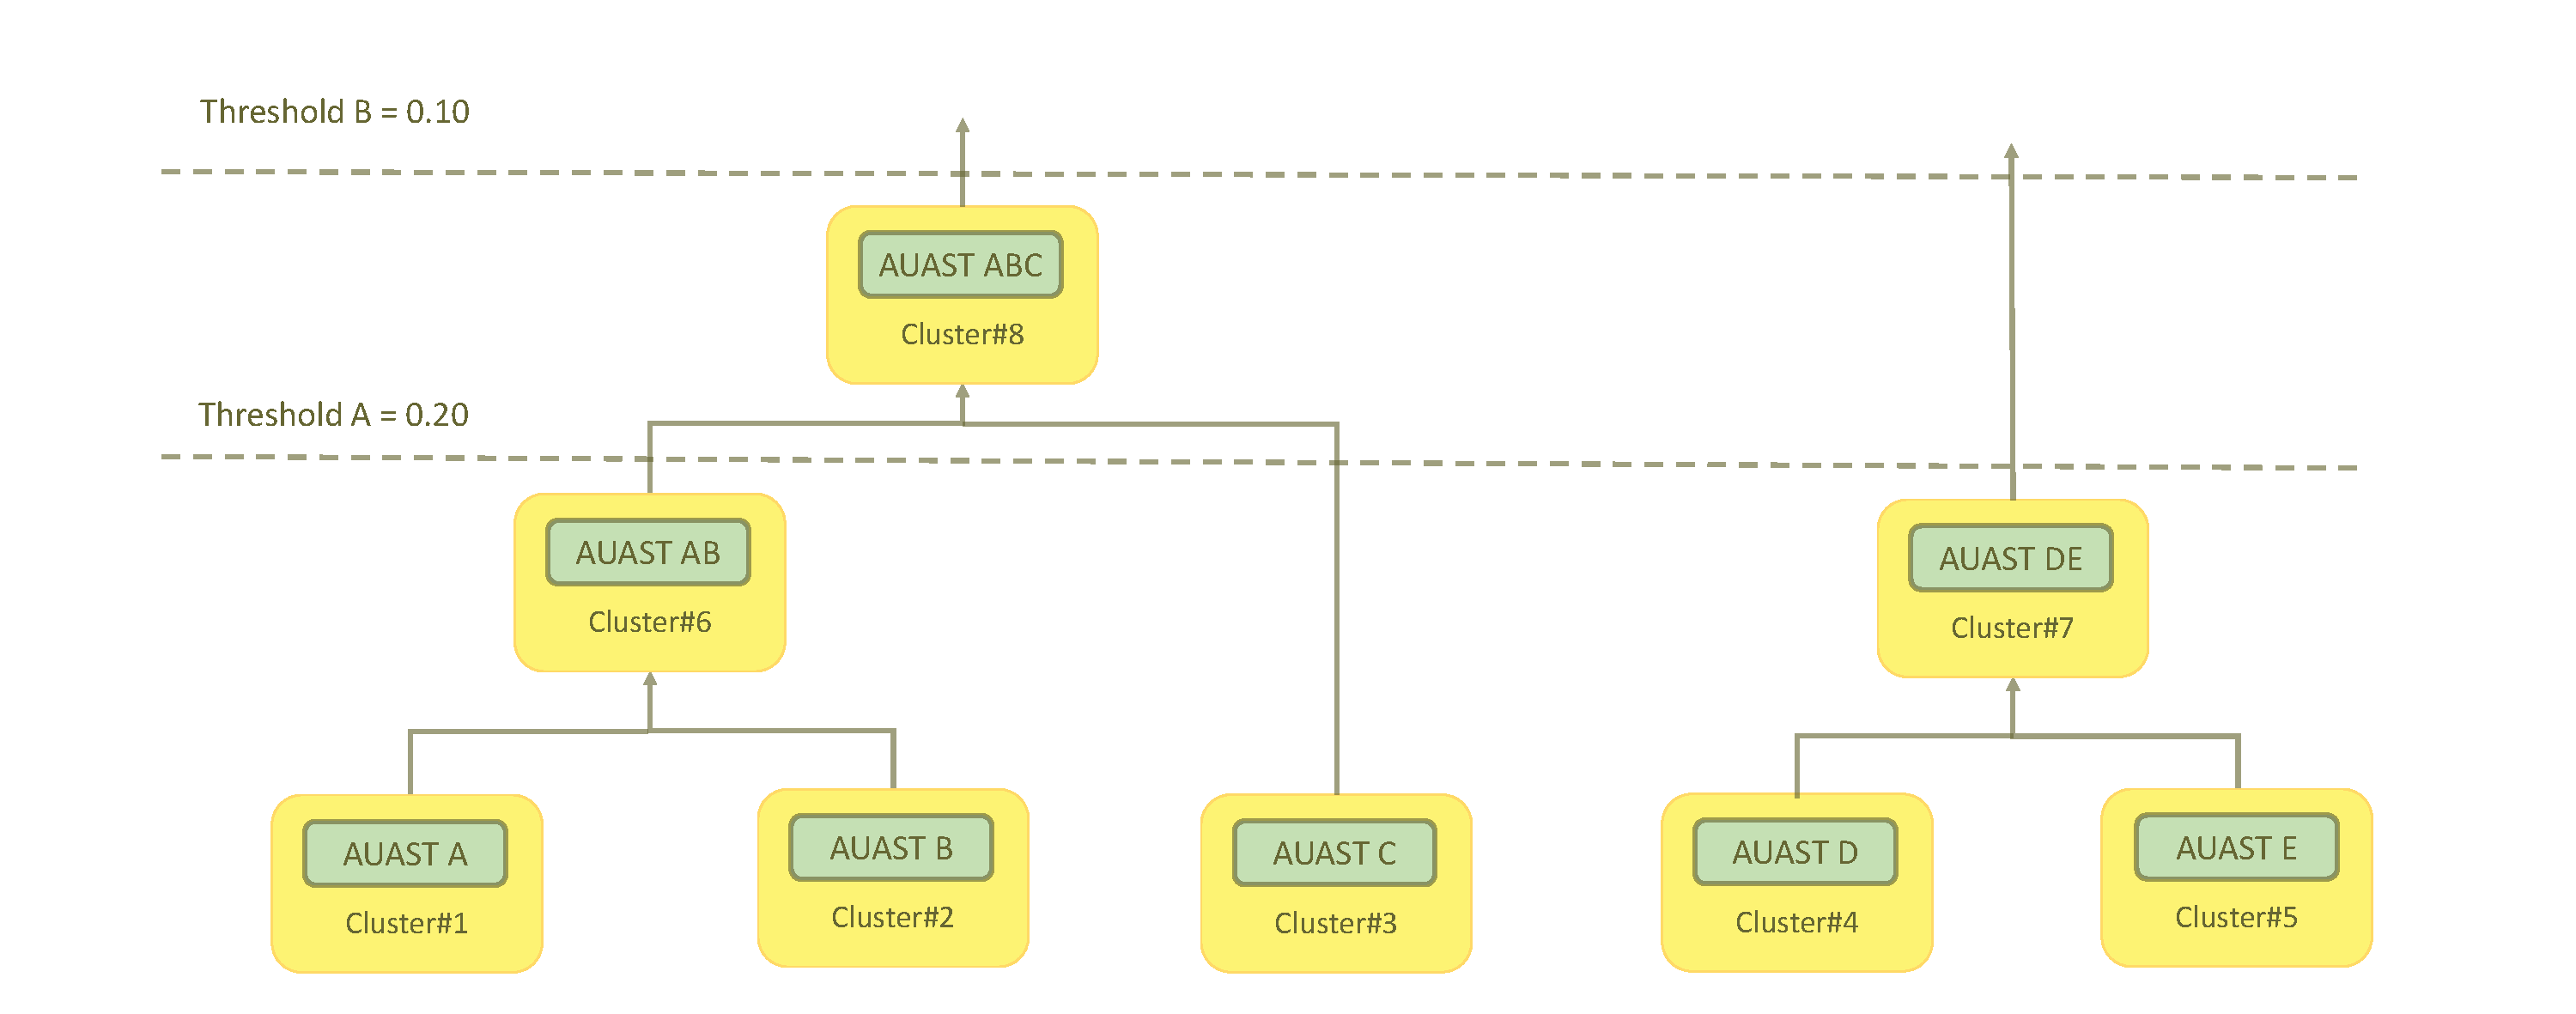
\includegraphics [width = \textwidth]{Drawing4/overview2.pdf}
  \caption{The agglomerative hierarchical clustering process for classifying 4 AUASTs. The threshold value indicates the number of clusters we will come up with.}
  \label{fig:overview2}
\end{figure}



%\RW{TBD}

\section{An Assessment of the Clustering tool}\label{clustering-assessment}
To assess the effectiveness of our clustering algorithm in classifying a set of AUASTs, we have implemented the clustering tool, which is a plug-in to the Eclipse integrated development environment (IDE), and conducted an experiment on the set of AUASTs of LJMs in the test suite described in Section~\ref{jigsaw-assessment}. The tool is developed atop the anti-unifier-building tool.

\subsection{Setup}  \label{study3-setup}
We manually attempted to perform the hierarchical clustering on the set of LJMs from the test suite and constructed the detailed anti-unifier view for each cluster. Anti-unifiers were discarded when the anti-unification of LJMs did not allow the anti-unification of logging calls with one another, as the Java elements enclosing them were not found to be corresponded. We also measured the level of similarity between LJMs in each cluster by computing the ratio of common Java elements in the detailed anti-unifier view to the total number of Java elements of all LJMs in that cluster. We also ran the clustering tool on the set of LJMs to classify them using the similarity measurement.

\subsection{Results}  \label{study3-results}
We present the results of our analysis in Table~\ref{results_clustering}. The analysis of the output has been divided into three categories: correspondence, similarity, and relevancy. The analysis of correspondence and similarity was described in Section~\ref{study2-results}. "Relevancy" represents that the usage of logging in Java methods of each cluster is similar that they should be grouped in the same cluster, and dissimilar to the other Java methods in the other clusters that should be scattered in different clusters. 

% "Relevancy" refers to the number of LJMs in each cluster that are detected to berelevant as their logging calls can be anti-unified with one another and cannot be anti-unified with logging calls of LJMs in the other clusters.
%AUASTs of all LJMs in each cluster

\begin{figure}
  \centering
  \begin{tabular}{|c|c|c|c|c|c|c|c|}
    \hline
  
    \multirow{2}{*}{Cluster}&\multicolumn{2}{c|}{Correspondence}&\multicolumn{2}{c|}{Similarity}&\multicolumn{2}{c|}{Relevancy}\\
    \cline{2-7}
    &Correct (\%)&Incorrect&human&tool&human&tool\\
    \hline
    1&28(100)&0&0.09&0.09  &4&4\\
    \hline
    3&24(92)&2&0.19&0.2& 3&3\\
    \hline
      2&9(100)&0&0.25&0.25& 3&3\\
 	\hline
  \end{tabular}
  \caption{Results from applying the clustering tool to the test suite.}
  \label{results_clustering}
\end{figure}

Our clustering tool succeeded in detecting the relevancy between the LJMs of our test suite. It also successfully calculated the similarity between LJMs of 2 clusters out of 3. In Cluster 2, the error in detecting correspondences originated from the previous study and propagated to the clustering study. However, it is trivial (0.01) and would have a low impact on our final results.

\section{Summary} \label{meth2-summary}
We have presented a modified version of the agglomerative hierarchical clustering algorithm to classify AUASTs of a set of LJMs using a measure of similarity. This algorithm is implemented as an Eclipse plug-in, which given a set of LJMs utilizes the anti-unifier building tool to measure similarities between AUASTs of each cluster pair and to construct an anti-unifier from them when two clusters need to be merged. Furthermore, an empirical study was conducted to evaluate the effectiveness of our clustering algorithm and its implementation in classifying AUASTs of the set of LJMs in our test suite.  
